\documentclass[12pt,a4paper]{report}

%------------------------------------------------------------------------
% PACKAGES:

\usepackage{lmtstyle}
% Define typearea
% a) Use automatic:
\usepackage[BCOR1cm]{typearea}
% b) Or use fixed:
%\usepackage{geometry}
%\geometry{left=1.5cm,textwidth=18.5cm,top=1.5cm,textheight=26.5cm}
\usepackage[american,ngerman]{babel}
% Use list of tabels, etc. in table of contents:
\usepackage{tocbibind}
% German paragraph skip
\usepackage{parskip}
% Encoder:????
\usepackage[latin1]{inputenc}
%\usepackage[applemac]{inputenc}
% Use A4-paper efficiently:
\usepackage{a4wide}
% Index-generation
\usepackage{makeidx}
% Einbinden von URLs:
\usepackage{url}
% Include .eps-files (needed also for the TUM-logo):
%\usepackage{epsf}
% Special \LaTex symbols (e.g. \BibTeX):
\usepackage{doc}
% Include Graphic-files:
%\usepackage{graphics}
% Include Graphic-files:
\usepackage{graphicx}
% Include doc++ generated tex-files:
%\usepackage{docxx}
% Include PDF links
%\usepackage[pdftex, bookmarks=true]{hyperref}
%------------------------------------------------------------------------
\usepackage{subfigure}
\graphicspath{{figures/}}

%########################################################################
% CHOOSE DEFAULT LANGUAGE:
%\setlang{de}
\setlang{en}

% FILL IN ACCORDINGLY:
\title{Refined Methods for Creating Tactile Signals respecting Speed Dependency}
\type{B} % / M:Master /B:Bachelor / F:Forschungspraxis / I:Ingenieurspraxis
\author{Irem �zt�rk}
\matrikelnr{03677343}
\street{Helene-Mayer-Ring 7A}
\town{80809 M�nchen}
\advisor{Matti Strese}
\datebegin{Datum des Arbeitsbeginns}
\dateend{Datum des Vortrags}
%########################################################################


\begin{document}%****************************************************

\makemtgtitle

% MAIN PART:
\pagenumbering{roman}
% German abstract:
\switchlanguage{de} % The Kurzfassung, if given, is supposed to be in German!

\thispagestyle{plain}

\section*{Kurzfassung} 
In der Kurzfassung werden auf einer halben Seite das Problemfeld und
die pr�sentierten Ergebnisse zusammengefasst.

\switchlanguage{\lang} % Switch back to the docmuent's default language.
% English abstract:
\switchlanguage{en} % The abstract is supposed to be in English!

\thispagestyle{plain}

\section*{Abstract}
%Titel auf Englisch wiederholen.

%Es folgt die englische Version der Kurzfassung.

\switchlanguage{\lang} % Switch back to the document's default language.
Several decades of research have been dedicated to the representation of real interactions in virtual or remote environments. Human-user studies form an integral part of the evaluation of haptic virtual systems. However, the drawback of  these  past approaches 
% Table of contents:
\tableofcontents 

% Introduction (Einleitung):

\chapter{Introduction}
\pagenumbering{arabic}%Ab hier, werden arabische Zahlen benutzt
\setcounter{page}{1}%Mit Abschnitt 1 beginnt die Seitennummerierung neu.
\thispagestyle{empty}
%Die Einleitung soll zum eigentlichen Themengebiet hinf�hren und die
%Motivation f�r die Arbeit liefern. Am Schlu� der Einleitung wird
%weiterhin noch eine �bersicht �ber die restliche Arbeit gegeben.

Scanning a textured surface with a tool generates rich high-frequency signals that describe mainly microscopic roughness of a surface. These captured vibrations are called vibrotactile or acceleration signals which is considered synonymous as in \cite{mouse18}.  To achieve full distal attribution, sensed vibrations must correspond to the user inputs in a physically appropriate manner \cite{Loomis92}.

A reasonable idea is that varying one's exploratory speed and normal force must significantly alter the
realism. However, studies (e.g. \cite{Culbertson15-WHC-Vibrations}) show that removing force responsiveness does not have a significant effect on the perceived  realism, whereas removing speed responsiveness is more salient to users. Therefore, vibration signals in this thesis include speed responsiveness and not force responsiveness.

Allowing texture vibrations to respond to user speed is a valuable part of creating realistic haptic textures, nonetheless can be a challenging and time consuming part of the implementation, if real recorded acceleration signals are displayed for every speed level. Some research \cite{romano10} elucidate mathematical models as an alternative solution for representing a vibration texture under specific probe-surface interaction conditions. 
 
This thesis has microscopic texture features as its center of focus and aims to evaluate the prediction results obtained from mathematical models, namely LPC and major frequency analysis, which are capable of reducing the size of stored models, to be able to display realistic vibrations at different speed levels through interpolated audio signals. 



% Text Body (Hauptteil)
% Could have multiple chaper-files, e.g.:
\thispagestyle{empty}
\cleardoublepage
\chapter{Haptic texture rendering}

\label{haptic}
\thispagestyle{empty}% no page number in chapter title page

The human haptic perception system relies on kinesthetic and cutaneous sensory information provided by several receptors during probe-surface interactions \cite{leder09}.
 
The kinesthetic sense focuses on the perception of forces and torques acting on the human
body. Kinesthetic stimulation is sensed by mechanoreceptors located in the muscles. Kinesthetic mechanoreceptors include muscle spindles in parallel with muscle fibers and Golgi tendon organs in series with them at the connection with the skeleton \cite{rahul15}. In some mainly kinesthetic tasks, the tactile sense only indicates a contact.

Tactile perception is stimulated by cutaneous receptors. There are four kinds of mechanoreceptors in the glabrous skin: The Merkel cells (Braille dots and sharp edges), Meissner corpuscles (low-frequency vibrations), Pacinian corpuscles (high frequency stimuli), Ruffini endings (still unknown).

Friction, hardness, macroscopic roughness, microscopic roughness and thermal conductivity are the main dimensions to build haptic texture models \cite{okamoto13}. All of these aspects should be well considered in order to increase immersion into a virtual environment. In the following of this thesis, microscopic roughness is our main focus as a vibrotactile feature.

Roughness plays an important role in haptic signal perception.The roughness dimension may be divided into two dimensions: macro and fine (micro) roughness as in \cite{okamoto13}.

\section{Macroscopic Roughness}

Due to the duplex nature of roughness,  macroscopic roughness should also be considered in order to understand fine roughness. As described in \cite{rahul15}, both of these surface features play a role in the haptic interaction. Coarse roughness is mainly represented by the ``uneven'', ``relief'', or ``voluminous'' labels, relevant with the visible height profiles of an object surface and mediated by different mechanisms from micro roughness.
The surface material structural threshold between coarse and fine textures was determined as approximately 200 microns \cite{finetexture}. For coarse surface roughness, the spatial  distribution of SAI units is related to roughness perception \cite{okamoto13}.

\section{Fine Roughness}

In the mechanism of fine roughness perception, FAI and FAII units contribute and is mainly represented by the ``rough" and ``smooth" labels. During surface-tool or surface-finger sliding motions, high frequency vibrations can be extracted using an accelerometer mounted on a human finger. Microscopic roughness impressions can be characterized by these vibrations. The macro and fine roughness dimensions can be separated according to the mentioned aspects but can intersect each other during the process of perception.  Figure \ref{fig:texture} illustrates the process of texture production with an accelerometer.
\begin{figure}[h!]
	\begin{center}
		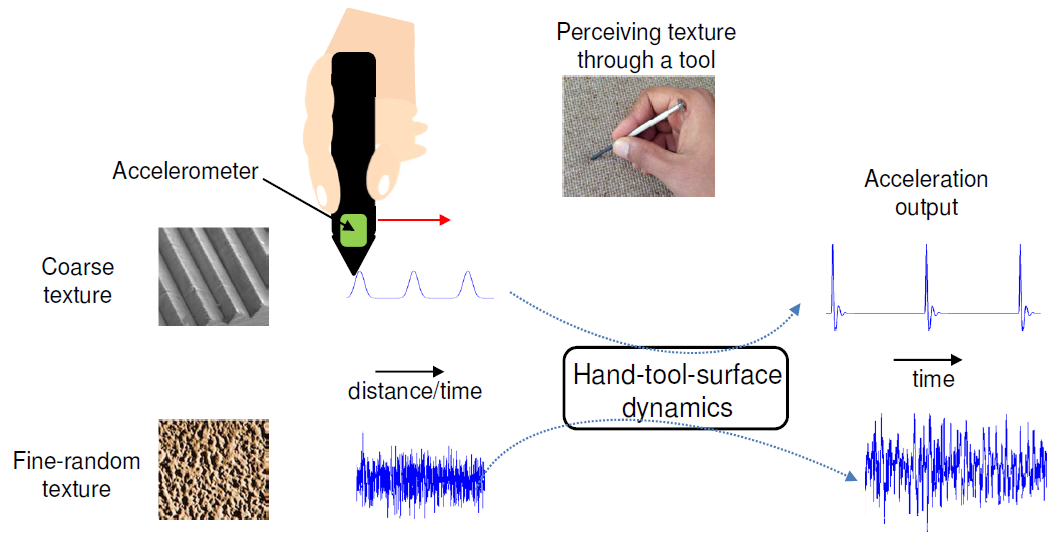
\includegraphics[width=14cm]{texture}
		\caption{Mechanism of texture production. A hand-held tool is used to stroke a textured surface. An acceleration sensor signal mounted on the tool measures the response of the hand-tool system as it hits surface features. Figure reproduced from \cite{rahul15} }
		\label{fig:texture}
	\end{center}
\end{figure}

The recorded acceleration signals depend on the scan speed and force, nonetheless we ignore the force dependencies as mentioned in the introduction part. Thereby, our approach in this thesis is generating vibrotactile signals based on the recorded acceleration data for different absolute scan speed. They are then displayed e.g. via a voice coil actuator. 


\chapter{Interpolation of vibrotactile signals}
\label{interpolation}
\thispagestyle{empty}
Prior model designs have recently been evolved into data-driven haptic textures. The apparent concept is simply displaying recorded texture acceleration signals, where the exploratory speed dependency is disregarded. However, this is not a sufficient way of representing acceleration response according to the human-subject studies during the past years (e.g. \cite{Culbertson15-WHC-Vibrations}) . Therefore, user speed should be incorporated into the feedback signal.

As in \cite{refined12} is described, there are some methods of relating speed variable to tactile signals such as switching between recordings according to speed, which may however be perceptually detectable. Another way is building a function depending on speed that gives a weighted average of recorded acceleration signals as output. The problem that may occur here is that the frequency content is not preserved due to the probable constructive and destructive interference between signals. These aspects create the idea of data-driven texture models.

In the following, we analyze two methods for synthesizing vibrotactile signals without creating noticeable artifacts. The first method is synthesizing two recorded acceleration signals under different speed conditions through LPC method and interpolating between them by linear interpolation of filter variables. The second one is reproducing these two signals from their major frequencies and interpolating between them to generate new signals.

In the following, we go deep into both of the principles and how to apply them to produce interpolated signals.

\section{Linear predictive coding}
\label{lpcmethode}
The basic idea of Linear Predictive Coding (LPC) is to develop a transfer function that can predict each sample of a signal as a linear combination of the previous samples. It has applications in filter design and speech coding. 

\begin{equation} \label{eq:sample}
\hat{x}[n]=\sum_{i=1}^{N}a_i \cdot x[n-i] 
\end{equation}

The equation \ref{eq:sample} above shows the prediction of a next value $\hat{x}[n]$ from the previous samples through LPC coefficients $a=[a_i]_{i=1:N}$, where N is the order of the filter.
The mean square prediction error is given as:

\begin{equation} \label{eq:errorfunctt}
E=\frac{1}{L}\cdot \sum_{k=1}^{L} {e[n]}^2  
\end{equation}

where L is the number of samples in the input signal and $e[n]=x[n]-\hat{x}[n]$.

For the implementation, we consider an IIR filter $H(z)$ of length n in the form $H(z)=[-h_1z^{-2}-h_2z^{-1}...-h_nz^{-n}]$.
Our acceleration data vector from PCA is called {$\vec{a}(k)$} in the following. The resulting prediction vector from our filter is $\vec{\hat{a}}(k)$. The residual signal {$\vec{e}(k)$} is the difference between these two signals as in the following equation:

\begin{equation} \label{eq:transferfunction}
\vec{e}(k)=\vec{a}(k)-\vec{a}(k) \cdot H(z)  
\end{equation}

\begin{equation} \label{eq:errorfunction}
\vec{e}(k)=\vec{a}(k)\cdot(1-H(z))   
\end{equation}
LPC Analysis filter $H(z)$ can be written as:

\begin{equation} \label{eq:transferfunct}
H(z)=1-P(z)   
\end{equation}

\begin{equation} \label{eq:transferfunctt}
P(z)=\frac{\vec{e}(k)}{\vec{a}(k)}   
\end{equation}

where $P(z)$ is described as the transfer function of the LPC filter.

It is possible to compute the residual at each step using the vector of filter coefficients $\vec{h}=[h_1 h_2 h_3 ... h_n]^T$:

\begin{equation} \label{eq:residual}
\vec{e}(k)=a(k)-\hat{a}(k)=a(k)-\vec{h}^T\vec{a}(k-1)  
\end{equation}

At this step, we aim to find the minimum value of the residual function $e(k)$. We are able to reduce the problem to Wiener-Hopf equation by a cost function based on mean-square error. The Wiener-Hopf equation can be solved by Levinson-Durbin \cite{durbin} algorithm, so that we can obtain our optimal filter vector $\vec{h_0}$. Levinson-Durbin determines by recursion the optimum ith-order predictor from the optimum (i-1)th-order predictor, and as part of the process, all predictors from beginning order (no prediction) to order p are computed along with
the corresponding mean-squared prediction errors E(i) (\cite{levinsondurbin}).

To synthesize new signals, we use a white noise signal {$\vec{e_g}(l)$} as input, which is filtered with $1/P(z)$, in order to generate our desired response {$\vec{a_g}(l)$}. For a better overview, we can rewrite the equations (\ref{eq:transferfunction}) and (\ref{eq:residual}) as follows:

\begin{equation}
\frac{\vec{a_g}(l)}{\vec{e_g}(l)}=\frac{1}{1-H(z)} =\frac{1}{P(z)} 
\end{equation}

\begin{equation}
a_g(l)=e_g(l)+\vec{h}^T\vec{a_g}(l-1) 
\end{equation}

Figure \ref{fig:lpc-blockdiagram} illustrates each of analyzing and synthesizing processes via block diagram. The value {$\vec{e_g}(l)$} is a randomly generated Gaussian white noise but its average signal power must be equal to that of the average signal power remaining in the residual, $P\{\vec{e}(k)\}$ after filter optimization.

\begin{figure} 
	\begin{center}
	\subfigure[Block diagram for prediction of the next contact acceleration $a(k)$
	given the recorded series $a(k)$ with residual $e(k)$.]{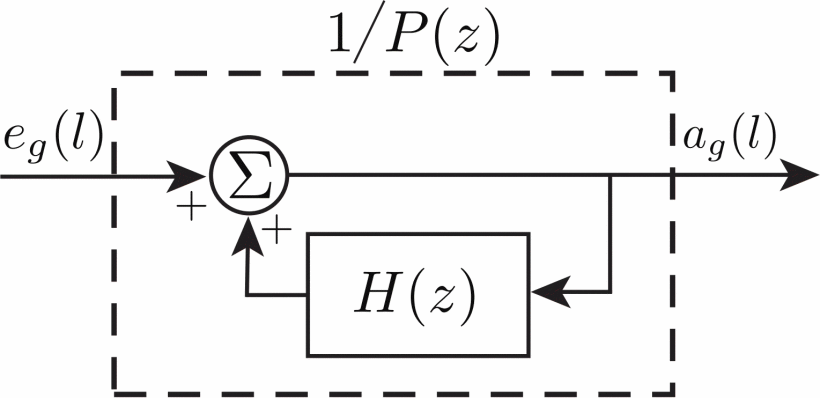
\includegraphics[width=0.49\textwidth]{lpcsynthesis}} 
	\subfigure[Block diagram for the synthesis of an acceleration signal $a_g(l)$
	from the appropriately scaled white noise input $e_g(l)$.]{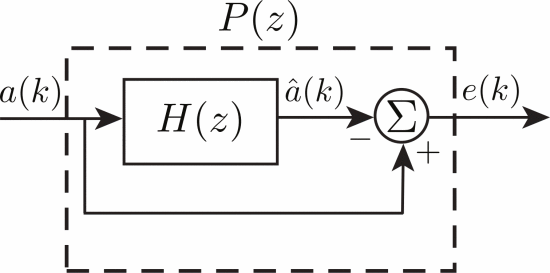
\includegraphics[width=0.49\textwidth]{lpc}} 
	\caption{Signal generation through LPC principle. Figures reproduced from \cite{romano10}.} 
	\label{fig:lpc-blockdiagram}
	\end{center}
\end{figure} 

The definition of power is as in the following equation:

\begin{equation}
P\{\vec{a}(l)\}=\frac{1}{N}\sum_{n=0}^{N-1}|a(n)|^2
\end{equation}

\begin{figure} [h!]
	\begin{center}
		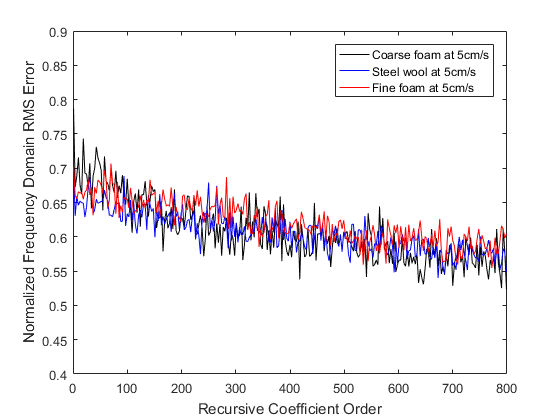
\includegraphics[width=0.70\textwidth]{error2} 
		
		\caption{The RMS Error of synthesized signals via LPC calculated with different coefficient orders. The original signals are recorded acceleration data at 5cm/s of materials oak, steel wool and fine foam. The chosen threshold is 400 as a result of this plot, where additional coefficients have minimal benefit.} 
		\label{fig:error2}
	\end{center}
\end{figure} 

This is equivalent to signal variance $\sigma�$, because our signals are zero-mean signals. Now, we have to determine the order of our prediction filter, which affect the accuracy of the prediction. The higher we choose the order, the smaller the residual gets. It means we have a better prediction with higher orders, but then the calculation gets  more complicated. It is possible to calculate the success of the synthetic result with a cost function defined as the RMS error (root mean square error) as follows:

\begin{equation} \label{costfunction}
C\{\vec{a_g}(l)\}=\frac{(DFT\{\vec{a}(l)\}-DFT\{\vec{\hat{{a_g}}}(l)\})_{RMS}}{(DFT\{\vec{a}(l)\})_{RMS}}
\end{equation}


where RMS and the discrete Fourier transform $DFT\{\vec{a}(l)\}$ of vector $\vec{a}(l)$ are defined as:

\begin{equation} \label{rms}
x_{RMS}=\sqrt{\frac{1}{n}({x_1}^2+{x_2}^2+...+{x_n}^2)}
\end{equation}

\begin{equation} \label{dft}
DFT\{\vec{a}(l)\}=\vec{A_k}(l)=\sum_{l=0}^{L-1}\vec{a}(l)\cdot e^{-2\pi kN}   \quad k=0,1,...N-1.
\end{equation}

Using this equation, it is possible to obtain the optimal order of the filter. As shown in Figure \ref{fig:error2}, the higher a coefficient order is chosen, the smaller gets the RMS error calculated via given formula. However, a major change in error value can not be seen among the orders higher than 400 as in \cite{romano10}, which is confirmed in Figure \ref{fig:error2}. That is why in this thesis 400 is chosen as the optimal order for the best quality of results.

\begin{figure} [htbp]
	\begin{center}
		\subfigure{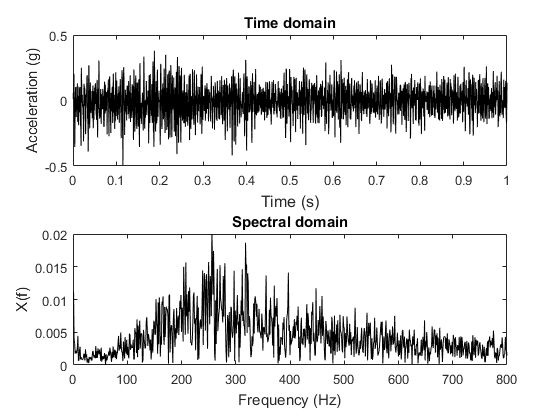
\includegraphics[width=0.70\textwidth]{gr_doppelt}} 
		\subfigure{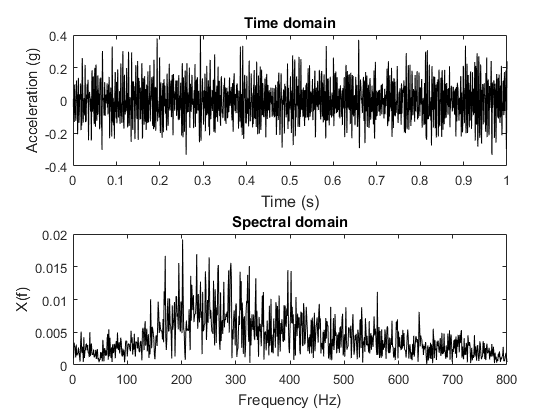
\includegraphics[width=0.70\textwidth]{gr_lpc}} 
		\caption{The upper plot shows the acceleration data recorded during interaction with a granite tile and its spectrum. The LPC synthesized version of the signal with the coefficient order 400 is shown in the second plot. Both signals maintain the same spectral characteristics, whereas they differ from one another in the time domain.}
		\label{fig:lpc-original}
	\end{center}
\end{figure} 


Now that we have generated our prediction filter with two unique variables $\vec{h}$ vector and $e_g(l)$, it comes to interpolate between our synthesized signals to create new signals. Bilinear interpolation of both the vector $\vec{h}$ and $e_g(l)$ of two signals in different velocities and applying these new values to our prediction filter result in new synthesized signals, so that signal data for audio signals at different force and velocities are created. For the interpolation of filter coefficients, we first convert them to line spectral frequencies (LSFs) to ensure stability during rendering \cite{modeling14}. Figure \ref{fig:lpc-original} shows an example signal and its LPC synthesized version both in time and spectral domain. 

The general feel of haptic textures is governed by their spectral signature \cite{haptography}. As in the figure \ref{fig:lpc-original}, the recorded and synthesized data differ on time-domain, but their spectrum are quite similar. So it is expected that they will feel the same to a user. Experiment I in chapter \ref{data} is going to deal with whether these correlations are strong enough to fool the human sense of touch.

\section{Signal Generation from Major Frequencies}
\label{majorfrequency}
The other method for signal generation is using rich and valuable information of signals' dominant frequencies, which has the highest amplitudes. The frequency of the vibration must change as the users change their force and so that their speed. This is one of the realistic methods for interpolation between signals recorded under different velocities.

At first we should determine the number of the frequencies we are going to deal with for synthesizing new signals. This is done as a part of Experiment I in chapter \ref{data} according to the participants' feedback. For our case we set 30 as the maximum number of selected frequencies and 2 as the minimum. The optimum will be evaluated with the aid of the first experiment.


\begin{figure} [htbp]
	\begin{center}
		\subfigure[30-31 Hz]{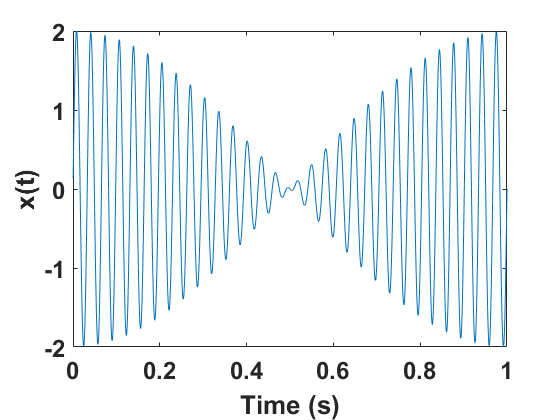
\includegraphics[width=0.30\textwidth]{schwebung1}} 
		\subfigure[80-81 Hz]{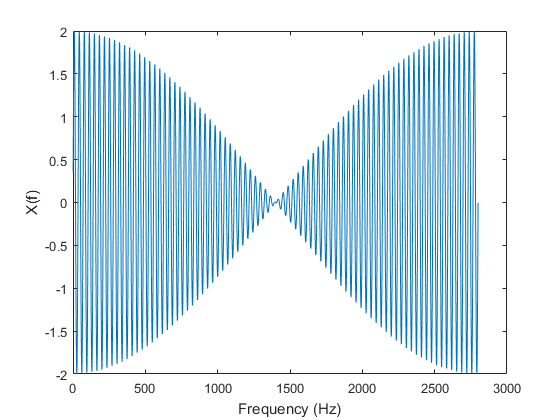
\includegraphics[width=0.30\textwidth]{schwebungg1}} 
		\subfigure[120-122 Hz]{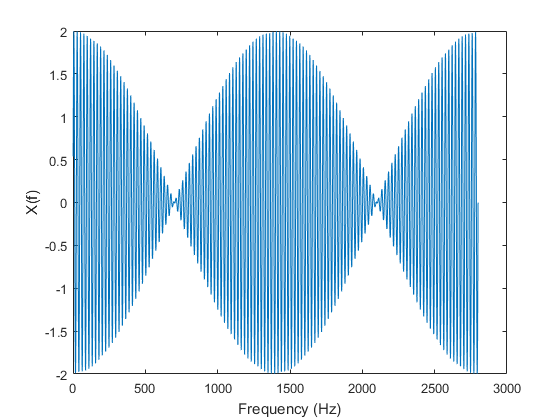
\includegraphics[width=0.30\textwidth]{schwebung31}} 
		
		\subfigure[30-32 Hz]{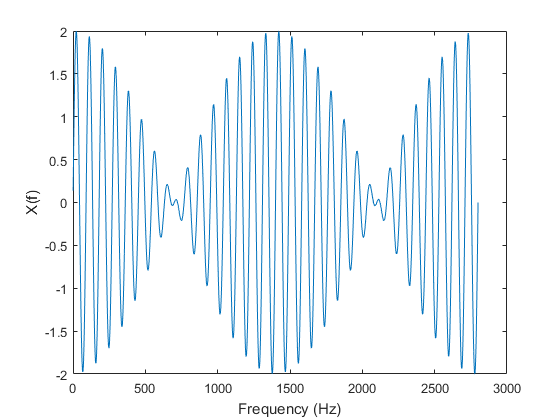
\includegraphics[width=0.30\textwidth]{schwebung2}} 
		\subfigure[80-82 Hz]{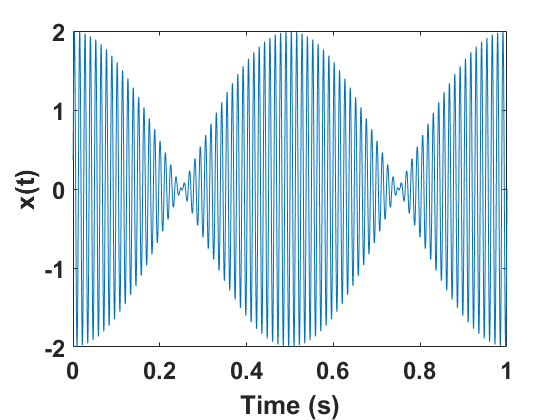
\includegraphics[width=0.30\textwidth]{schwebungg2}} 
		\subfigure[120-124 Hz]{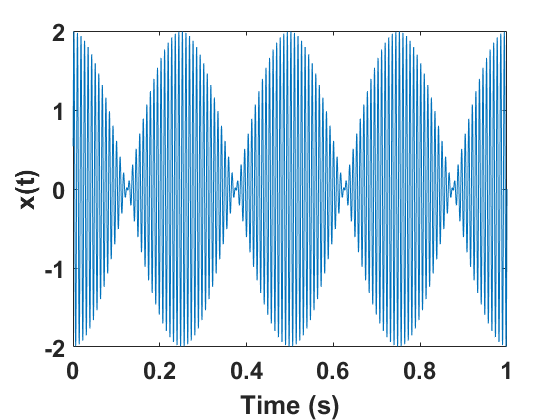
\includegraphics[width=0.30\textwidth]{schwebung32}} 
		
		\subfigure[30-33 Hz]{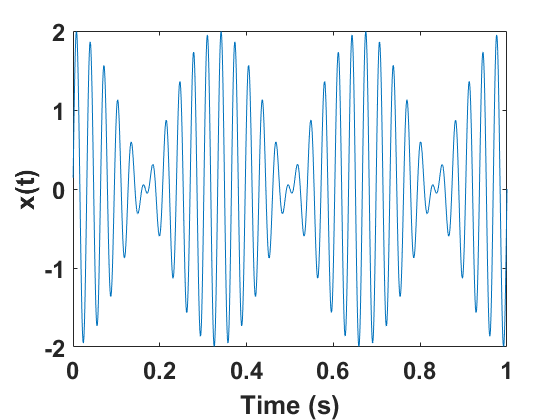
\includegraphics[width=0.30\textwidth]{schwebung3}} 
		\subfigure[80-83 Hz]{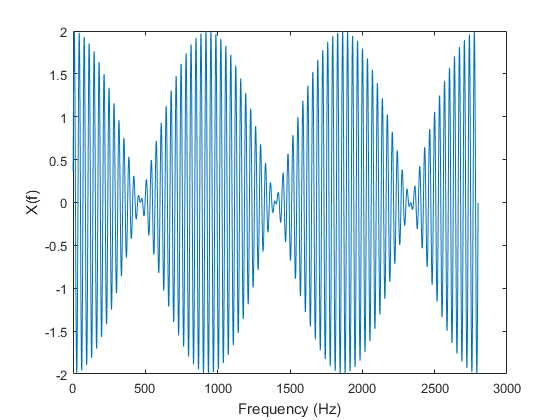
\includegraphics[width=0.30\textwidth]{schwebungg3}} 
		\subfigure[120-126 Hz]{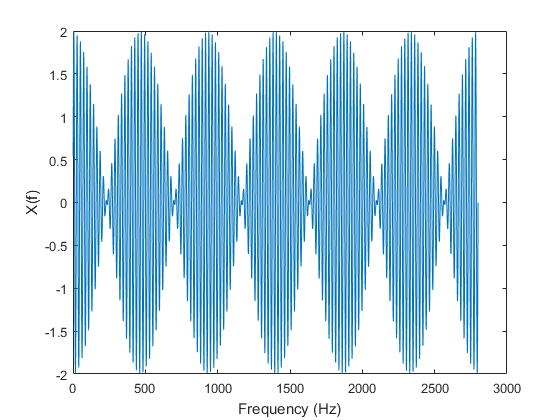
\includegraphics[width=0.30\textwidth]{schwebung33}}
		\subfigure[30-34 Hz]{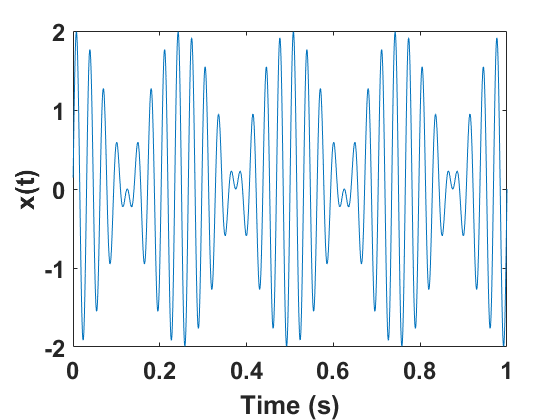
\includegraphics[width=0.30\textwidth]{schwebung4}} 
		\subfigure[80-84 Hz]{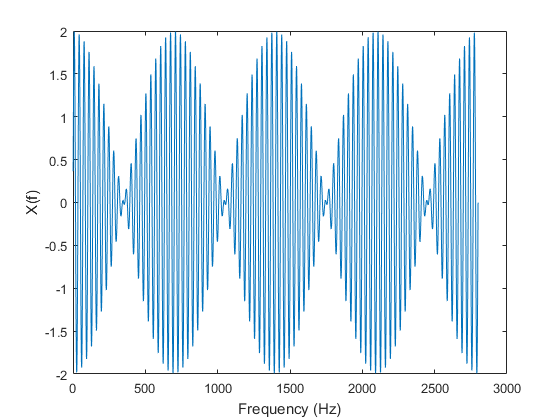
\includegraphics[width=0.30\textwidth]{schwebungg4}}
		\subfigure[120-128 Hz]{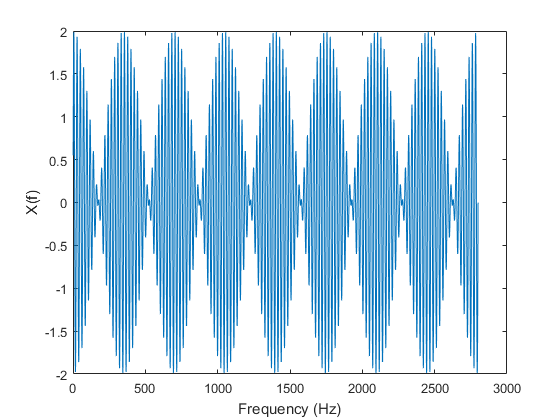
\includegraphics[width=0.30\textwidth]{schwebung34}}
		\subfigure[30-35 Hz]{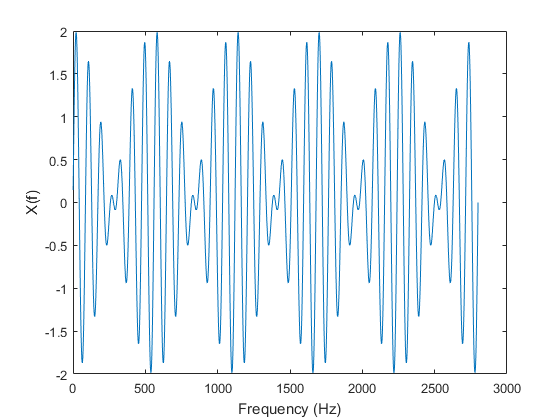
\includegraphics[width=0.30\textwidth]{schwebung5}}
		\subfigure[80-85 Hz]{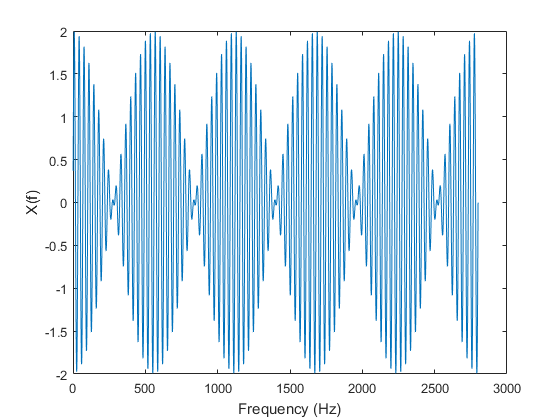
\includegraphics[width=0.30\textwidth]{schwebungg5}}   
		\subfigure[120-130 Hz]{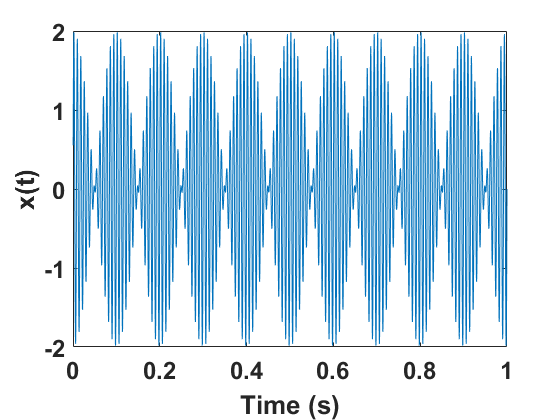
\includegraphics[width=0.30\textwidth]{schwebung35}}
		
		  \caption{The plotted signals are generated as a summation of two periodic signals, which have the frequencies given below respectively, in order to observe the threshold distance for the beats wave.} 
		\label{fig:schwebung}
	\end{center}
\end{figure} 

\begin{figure} [htbp]
	\begin{center}
		\subfigure[170-172 Hz]{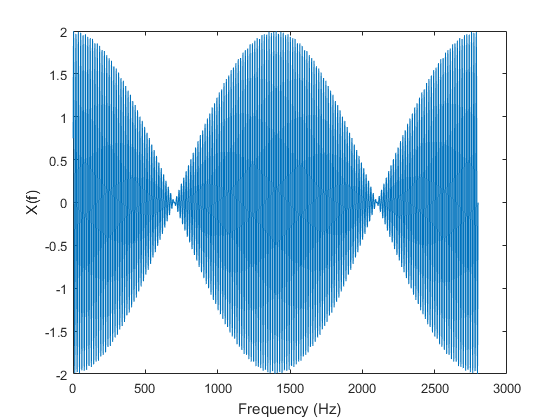
\includegraphics[width=0.30\textwidth]{schwebung41}}
		\subfigure[300-304 Hz]{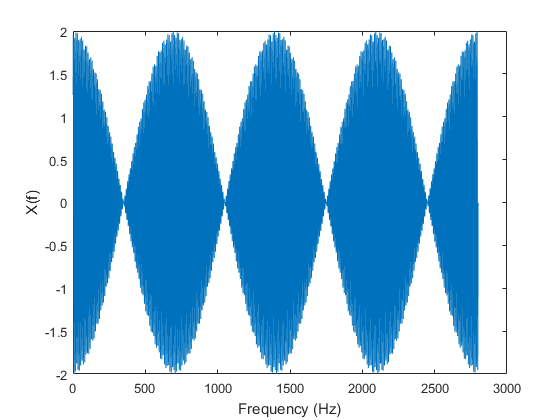
\includegraphics[width=0.30\textwidth]{schwebung51}}
		\subfigure[500-530 Hz]{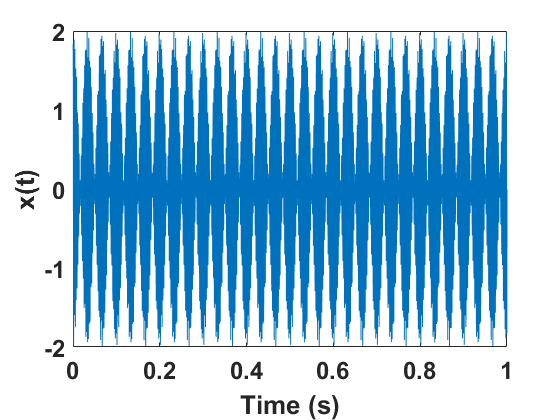
\includegraphics[width=0.30\textwidth]{schwebung61}}
		\subfigure[170-174 Hz]{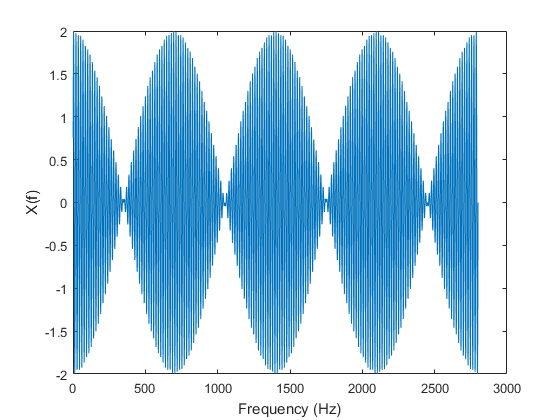
\includegraphics[width=0.30\textwidth]{schwebung42}}
		\subfigure[300-308 Hz]{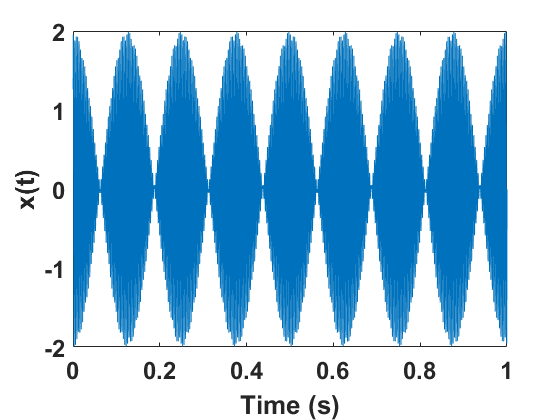
\includegraphics[width=0.30\textwidth]{schwebung52}}
		\subfigure[500-560 Hz]{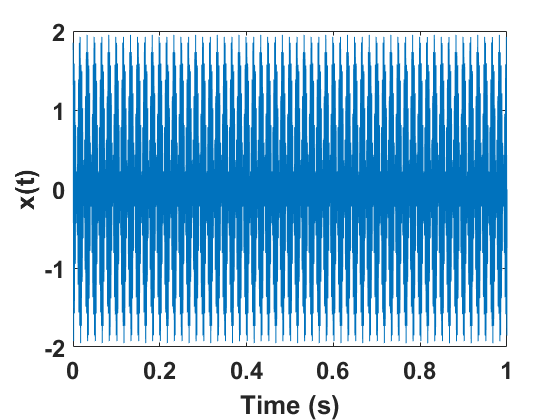
\includegraphics[width=0.30\textwidth]{schwebung62}}
		\subfigure[170-176 Hz]{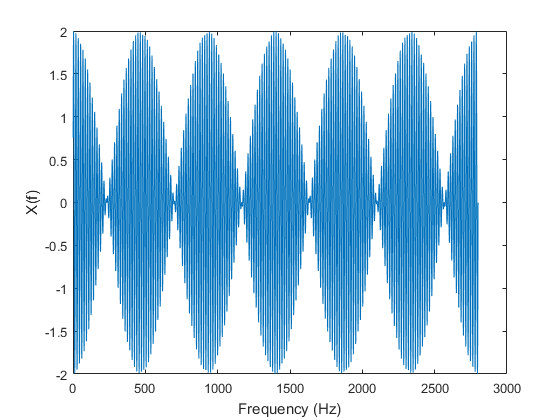
\includegraphics[width=0.30\textwidth]{schwebung43}}
		\subfigure[300-312 Hz]{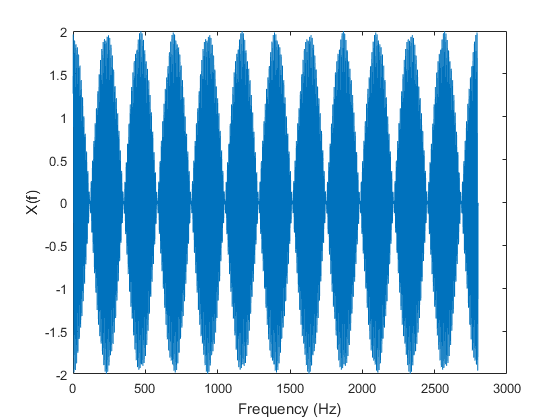
\includegraphics[width=0.30\textwidth]{schwebung53}}
		\subfigure[500-590 Hz]{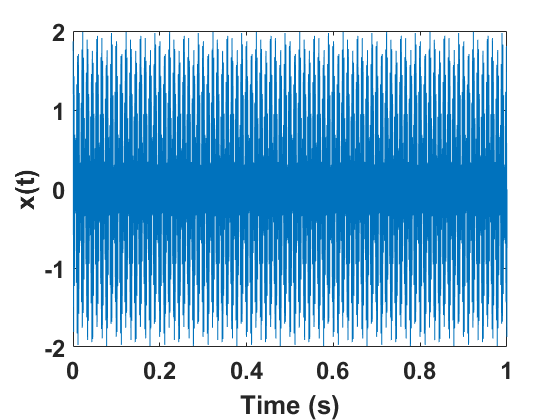
\includegraphics[width=0.30\textwidth]{schwebung63}}
		\subfigure[170-178 Hz]{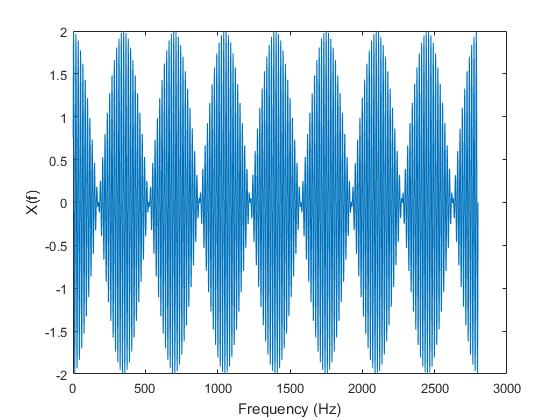
\includegraphics[width=0.30\textwidth]{schwebung44}}
		\subfigure[300-316 Hz]{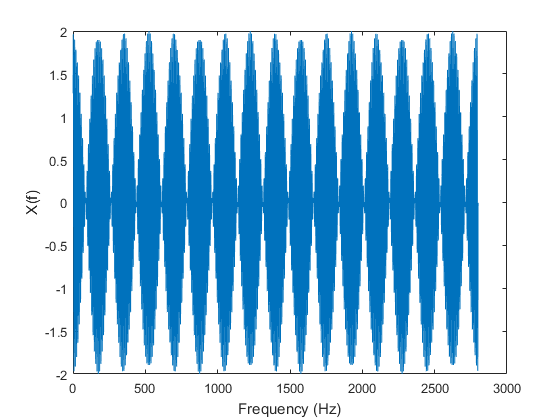
\includegraphics[width=0.30\textwidth]{schwebung54}}
		\subfigure[500-620 Hz]{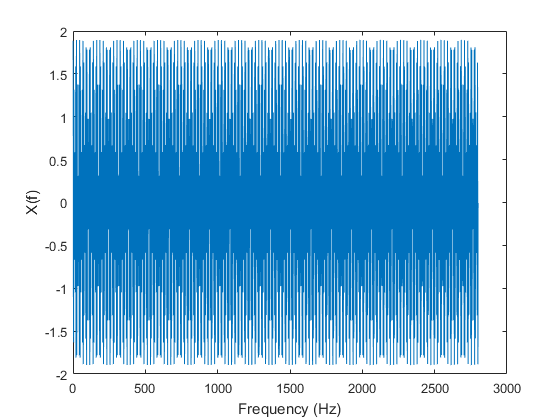
\includegraphics[width=0.30\textwidth]{schwebung64}}
		\subfigure[170-180 Hz]{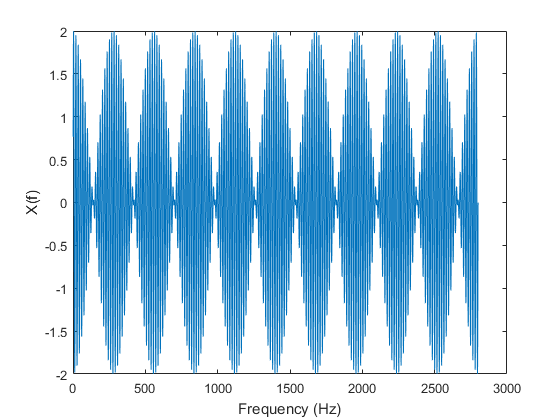
\includegraphics[width=0.30\textwidth]{schwebung45}}
		\subfigure[300-320 Hz]{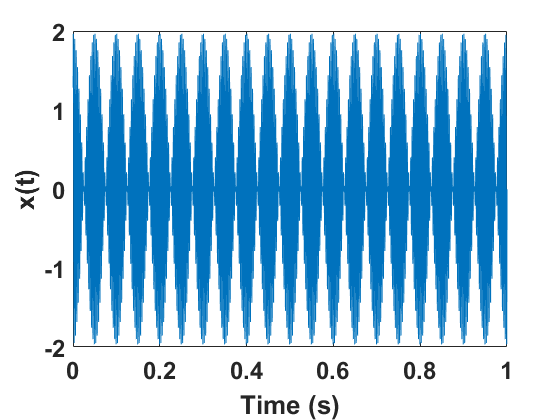
\includegraphics[width=0.30\textwidth]{schwebung55}}
		\subfigure[500-650 Hz]{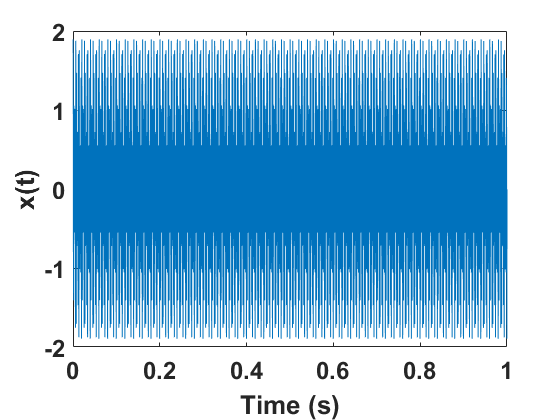
\includegraphics[width=0.30\textwidth]{schwebung65}}
		
		\caption{The plotted signals are generated as a summation of two periodic signals, which have the frequencies given below respectively, in order to observe the threshold distance for the beats wave.}  
		\label{fig:schwebung2}
	\end{center}
\end{figure} 


In order to find the frequencies with highest amplitudes, we calculate the discrete Fourier transform of the two recorded data and then select highest amplitudes of the transformed signals with the following equations:

\begin{equation}
T=\frac{1}{f_s}
\end{equation}
\begin{equation}
t=k\cdot T			\quad k=0,1...N-1
\end{equation}
\begin{equation}
X(f)=DFT\{x\}
\end{equation}

where N is the length of our input $x$. $X(f)$ is defined as the discrete Fourier transformed of the signal $x$ and contains therefore complex numbers in the form of ${\displaystyle z=r(\cos \varphi +i\sin \varphi )}$, where r is the amplitude and $\varphi$ describes the phase of the complex number. To be able to find the maximum amplitudes of $X(f)$, we determine all the amplitudes of X(f) with $abs(X(f))$ function and save also the phases for synthesizing new signals afterwards with $phase(X(f))$ function in Matlab. 

It is important here to ensure that selected frequencies should have a certain distance to each other, because the superposition of two pure tones with slightly different frequencies can lead to beats. The resulted wave is observed as a very low frequency of $\delta f$ and can be felt by the human tactile or auditory sense as if there is another stimulation \cite{beats}. To avoid this phenomenon, we remove frequencies among selected ones with a small difference.

The threshold difference that the frequencies should have among each other is not the same in low and high frequency range as described in \cite{rahul15}. In this thesis the intervals and their threshold differences are determined according to an artificial signal generated by two frequencies, which are selected closer step by step (see Figures  \ref{fig:schwebung} and \ref{fig:schwebung2}) and the experiment results in \cite{beats}, which allow us to find appropriate frequency intervals and their threshold frequency. However, due to the fact that there is not a fix value in literature for how close should these frequencies be selected and it is hard to , an evaluation was carried out with 5 people (3 female and 2 male between 22-28 years old, all right-handed), in order to achieve the optimal threshold for the model described in this thesis. 

\subsubsection*{Evaluation of Threshold Difference}

The subjects were asked to evaluate, whether they feel the beats signal in the audio signals displayed via a voice coil actuator with their right index finger. The signals were generated as in Figures \ref{fig:schwebung} and \ref{fig:schwebung2} from two frequencies, which have the maximum distance 20 in interval of 30-500 Hz and 150 in 500-1400 Hz. The threshold difference for each subject, where they began to percept the beats sensation can be seen in the following tabular \ref{tab:matrix}:

\begin{table}[htbp]
	\begin{center}
		\caption{The threshold differences, which are determined by the subjects, according to the perception of the beats sensation are given below. The signals were displayed respectively, beginning with the signals generated from the frequencies with the maximum distance, which gets smaller step by step, until the subject feels the beats signal.}
		\begin{tabular}{|c||c|c|c|c|c|}
			\hline 
			Frequency interval in Hz & Person I & Person II & Person III & Person IV & Person V  \\ 
			\hline 
			\hline
			$0-50$ &4  &6  &6  & 5 & 3  \\ 
			\hline 
			$50-100$ &5  &7  & 6 & 4 & 3 \\ 
			\hline 
			$100-150$ &6  & 9 & 9 & 7 & 6   \\ 
			\hline 
			$150-250$ &7  & 9 & 7 & 7 & 7   \\ 
			\hline 
			$250-500$ &15  &12  & 15 &15  & 14  \\ 
			\hline 
			$500-1400$ &60  & 30 &80  &30  & 30   \\ 
			\hline 
		
		\end{tabular} 
		\label{tab:matrix}
	\end{center}
\end{table}

This experiment also proves the fact that, the higher frequencies are more sensible for beats perception than lower frequencies. For a stable result, the major frequencies are selected according to the biggest threshold difference percepted by the subjects. The resulting values for each interval are shown in tabular  \ref{tab:threshold}.  

\begin{table}[htbp]
	\caption{The frequencies are selected from given intervals and have the threshold difference among each other.}
	\begin{center}	
		
		\begin{tabular}{||c c||} 
			\hline
			Frequency interval in Hz & Difference threshold in Hz \\ [1ex] 	
			\hline\hline
			0-50  & 6   \\ 
			\hline
			50-100 & 7  \\
			\hline
			100-150 & 9  \\
			\hline
			150-250 & 9  \\
			\hline
			250-500 & 15 \\  
			\hline
			500-1400 & 80 \\  
			\hline
		\end{tabular}
		\label{tab:threshold}
	\end{center}
\end{table}


In Figures \ref{fig:co1_1} and \ref{fig:co1_2}, an example of oak material is shown to illustrate how the artificial signal is generated from the recorded data. The signal is recorded at a very slow scanning speed (50mm/s) on oak and the obtained three-axis time-domain signals are reduced to one-axis using DFT321 \cite{romano12}. The generated signal from selected frequencies is in Figure \ref{fig:co1_3} both in time and spectral domain. 

\begin{figure} [htbp]
	\begin{center}
	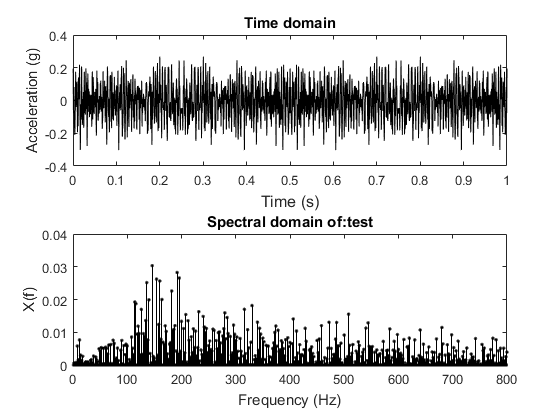
\includegraphics[width=0.70\textwidth]{co1_1} 
	 
	\caption{The depicted signal is recorded during an interaction with oak at a speed of 40 mm/s. The first plot shows the reduced one-axis signal in time domain and second plot shows spectral properties of the signal.} 
	\label{fig:co1_1}
		\end{center}
\end{figure} 

\begin{figure} [htbp]
	\begin{center}
		
	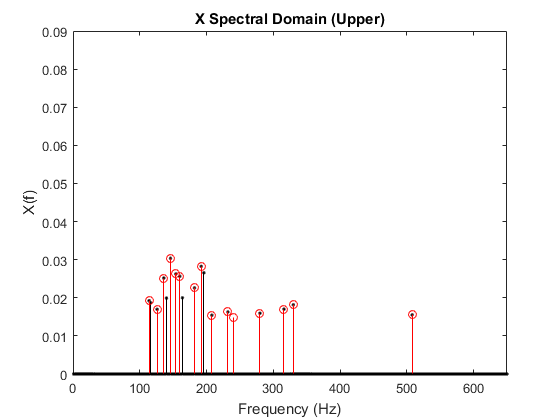
\includegraphics[width=0.70\textwidth]{co1_2} 

\caption{As shown in this example, the red points show the 30 selected frequencies and the black ones demonstrate the frequencies, which have amplitudes higher than the half of the maximum amplitude of the signal. Thus, the upper side of the spectral domain is shown with selected frequencies for a better overwiev.} 
\label{fig:co1_2}
\end{center}
\end{figure} 

\begin{figure} [htbp]
	\begin{center}
		\subfigure{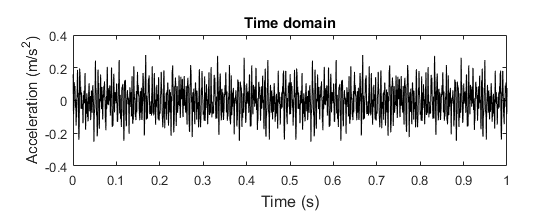
\includegraphics[width=0.70\textwidth]{co1_time}} 
		\subfigure{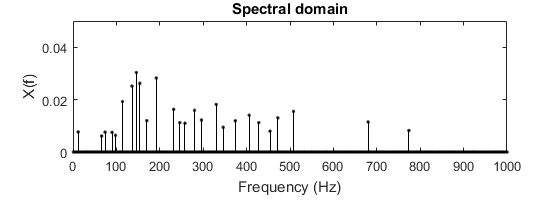
\includegraphics[width=0.70\textwidth]{co1_spectrum}} 
	\caption{First plot is the time domain of the generated signal via the frequencies in the second plot, which were chosen in Figure \ref{fig:co1_2}.}
	\label{fig:co1_3}
	\end{center}
\end{figure} 


The selected frequencies of the recorded signals are utilized for generating new signals. We determine the angle and the amplitude of each selected frequency before the generation process. We synthesize new signals by applying linear interpolation to the selected frequencies' amplitudes (see Figure \ref{fig:major}) and new signals are generated according to the following equation:


\begin{equation} \label{synthesize}
X_S(\hat{f})=\hat{A} \cdot e^{\hat{P}\cdot j}
\end{equation}

\begin{figure} [htbp]
	\begin{center}
		\subfigure[First generated signal from recorded data during interaction with oak at speed 40mm/s reproduced from given frequencies below.]{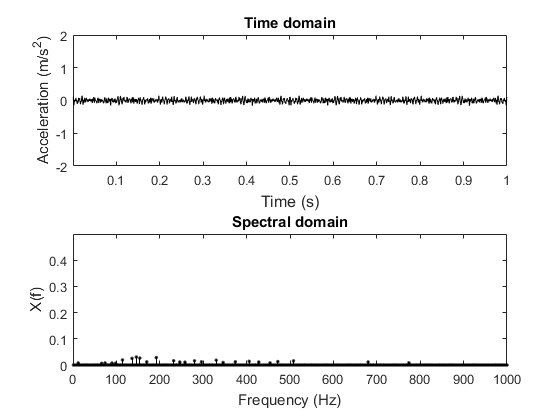
\includegraphics[width=0.80\textwidth]{coak1}} 
		\subfigure[An interpolation result between signals in (a) and (d).]{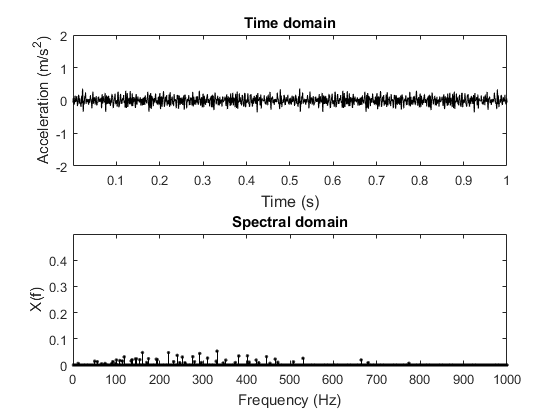
\includegraphics[width=0.80\textwidth]{coak5}} 
		
		\label{fig:major}
	\end{center}
\end{figure} 
\begin{figure} [htbp]
	\begin{center}
		
		\subfigure[Another result of the interpolation. Combination of the frequencies can be seen in the spectral domain plot below.]{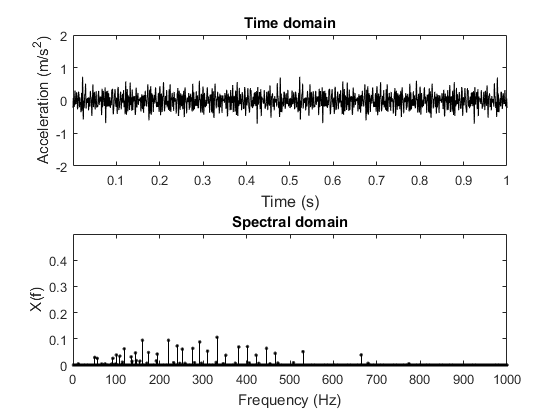
\includegraphics[width=0.80\textwidth]{coak7}} 
		\subfigure[The reproduced signal from recorded data at speed 400mm/s reproduced from given frequencies below.]{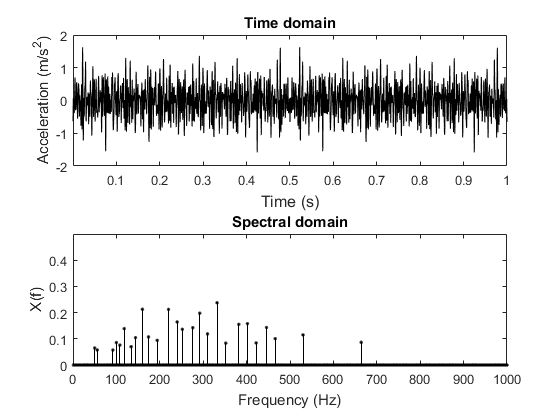
\includegraphics[width=0.80\textwidth]{coak10}} 
		\caption{Signal interpolation through frequencies with highest amplitudes.} 
		\label{fig:major2}
	\end{center}
\end{figure} 


where $\hat{A}$ represents the amplitude of selected frequencies $\hat{f}$ and $\hat{P}$ represents the phase of selected frequencies with k as the selected frequency order. Signal $X_S$ is the generated spectrum, which needs to be transformed into the time domain (see Figure \ref{fig:co1_3}) via IFFT to get the estimated signal via the following equation: 

Finally in both methods, we generate audio signals by $audiowrite$ function in Matlab, which are displayed during interactions with virtual surfaces.

\chapter{Correlation of Friction and Scanning Speed }
\label{friction}

Surface stickiness compels the users to apply a lateral force during surface interactions. The friction coefficient is usually calculated as the ratio
of the required dragging force of a sensor to the pressure, or
normal force \cite{mouse18}. 

\section{Speed Test}
In the following, we use Novint Falcon haptic device to feel a surface with different friction conditions, to be able to create a speed scala for some friction coefficients. Our aim is demonstrating how user speed varies depending on friction coefficients. We then use these results to evaluate speed intervals to be created in the following of this thesis, in which different audio data is displayed.

The test is carried out with an object in a haptic virtual environment, which has no friction at the beginning. The object surface to be explored was a $20 \times 20$ $cm^2$ square. The scanning speed is detected and saved in every 0.2 seconds, while the user explores the surface. Approximately after one minute, system automatically changes the friction and brings it to one level higher. The friction coefficients and the results are shown in Figures \ref{fig:boxplot} and \ref{fig:friction}.

\begin{figure} [htbp]
	\begin{center}
		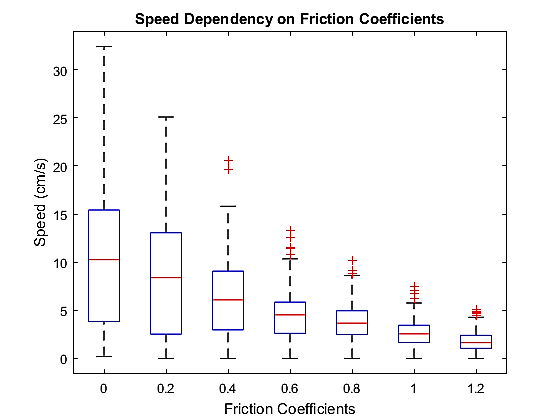
\includegraphics[width=0.70\textwidth]{boxplot} 
		
		\caption{Boxplot between friction coefficients of a virtual surface and speed values detected in every 0.2 seconds.} 
		\label{fig:boxplot}
	\end{center}
\end{figure} 

\begin{figure} [htbp]
	\begin{center}
		\subfigure[]{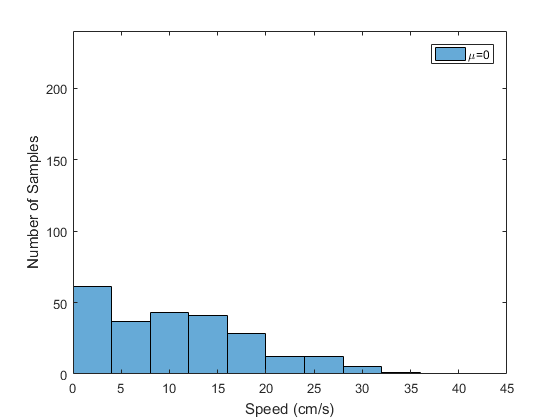
\includegraphics[width=0.40\textwidth]{hist1}} 
		\subfigure[]{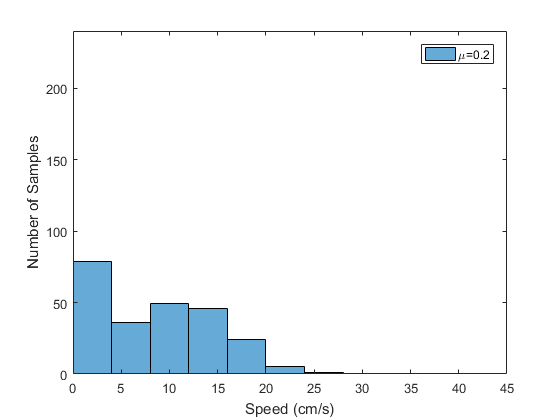
\includegraphics[width=0.40\textwidth]{hist2}} 
		\subfigure[]{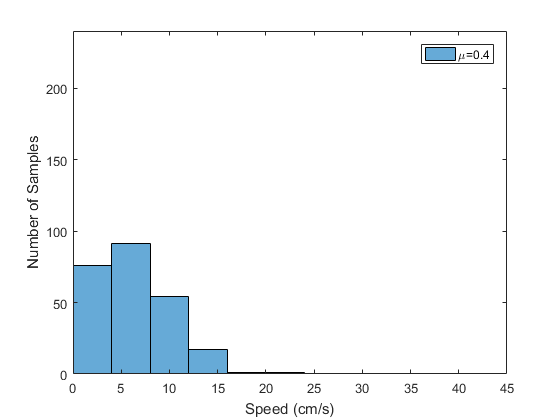
\includegraphics[width=0.40\textwidth]{hist3}} 
		\subfigure[]{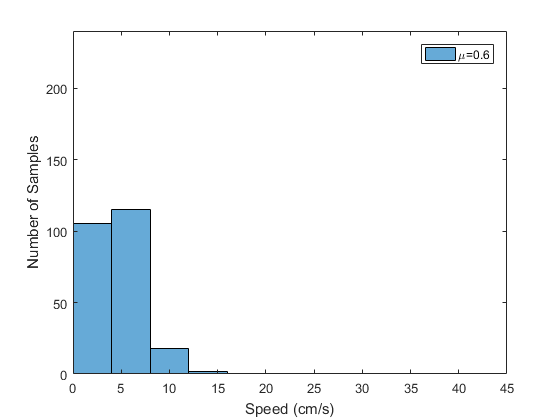
\includegraphics[width=0.40\textwidth]{hist4}} 
		\subfigure[]{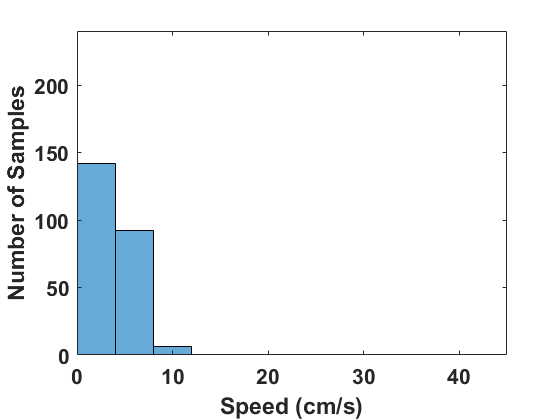
\includegraphics[width=0.40\textwidth]{hist5}} 
		\subfigure[]{\includegraphics[width=0.40\textwidth]{hist6}} 
		\subfigure[]{\includegraphics[width=0.40\textwidth]{hist7}} 
		\caption{Histograms of each 7 friction coefficients with 240 speed samples saved in every 0.2 seconds during virtual surface interaction through a haptic device.The bin width is selected as 4 in each plot.}  
		\label{fig:friction}
	\end{center}
\end{figure} 


\section{Evaluation}

Figure \ref{fig:boxplot} presents the mean speed value and the common speed interval for each coefficient order. As expected, both the speed interval and the mean value get smaller with increasing friction coefficient. Figure \ref{fig:friction} gives us hints to be able to analyze how many intervals there are to display different audio data to simulate real surfaces.

In plot (a), nine bins are shown, where the last two can be ignored due to the small number. So in that case, we would choose seven intervals for changing audio as the user speed varies, on the other hand in real life, textures always have a friction above zero, so this example depicts an unnatural scenario. When we look at the most common coefficients like 0.2 and 0.4, which are also relevant for the experiments in following chapters, we recognize that, it is possible to work with less than seven intervals for vibrotactile response. In the case of 0.2, five bins are remarkable as peaks and the rest can be part of the last interval. For the friction 0.4, we can assign four intervals and for 0.6 three audio data are quite sufficient. The fine roughness of objects with 0.8 and 1.0 friction coefficient can be displayed with two signals and for the last and extreme case one audio is enough already according to the presented results, so that there is no need to interpolate the recorded data.



\chapter{Data-Driven and Frequency Reduction Methods for Tactile Signal Evaluation}
\label{data}

The perception of displayed haptic
information typically varies across different human subjects \cite{leder09}. Therefore,experiments with human participants and their feedbacks constitute a fundamental component of the development in haptics.

As mentioned in chapter \ref{interpolation}, we analyze two methodologies of synthesizing vibrotactile signals for rendering fine roughness feedback: LPC and utilizing major frequencies of records. This chapter describes a human-subject experiment to evaluate how perceptually close our synthesized vibrotactile signals to the recorded acceleration signals in a haptic environment.  

\section*{Experiment I}

\section{Subjects and Setup}
\label{subjects}

To accomplish a stable evaluation, ten volunteer human subjects, 3 female and 7 male, participated in the experiment at separate times. Their
ages ranged from 19 to 29, with an average of 23 years. The subjects were all right-handed with limited experience with haptic devices. None
of them reported having any ailments that would affect the experiment.

We used the voice coil actuator model NCC01-04-001-1X by H2W Technologies in the experiment to display vibrotactile signals. 5 objects were relevant for this experiment as shown in the tabular \ref{tab:materials}.
\begin{table}[htbp]
		\caption{Materials in the experiment given with their approximated friction coefficients.}
\begin{center}	
	
	\begin{tabular}{||c c||} 
		\hline
		Material & Friction \\ [1ex] 	
		\hline\hline
		Coarse foam & 0.6   \\ 
		\hline
		Fine foam & 0.6  \\
		\hline
		Oak & 0.2  \\
		\hline
		Granite Tile & 0.2  \\
		\hline
		Steel wool & 0.4 \\  
		\hline
	\end{tabular}
	\label{tab:materials}
\end{center}
\end{table}



\section{Procedure}

The subject sat at a table in front of the voice coil actuator. In each experiment run, the subject compared a synthesized signal with the reference while perceiving the response with the right index finger. The displayed reference signal was for each material a recorded acceleration data at the mean speed according to the results in Figure \ref{fig:friction} in chapter \ref{friction} and the compared synthesized signal was reproduced from this data both via LPC and major frequency method. 

In addition to LPC and major frequency methodologies, the signal obtained by converting the initial signal from time domain to frequency domain via DFT and then converting back from the frequency domain to the time domain via IFFT was also displayed to be compared with the reference by the participants. The intent here is to remove possible peculiarities that may have occurred at the beginning and end of the recording and so that providing a stable signal from the recording. 

The subject was supposed to compare each pair of signals respectively and evaluate whether they cause the same or different perception. Before each synthesized signal, the recorded signal is displayed for 10 seconds. Afterwards the artificially generated audio is displayed again for 10 seconds and the participant was asked to evaluate directly. Hereby, all methods were judged regarding to the reference.

Another important aspect of this experiment is to find the optimum number of frequencies to be selected experimentally as mentioned in section \ref{majorfrequency}. To do this, the synthesized data via 2 to 30 selected frequencies for all materials were prepared to display. We always started with the signal created with 30 frequencies and if the user can not detect any difference between the reference and comparison vibration, the 2-frequency signal was displayed. Gradually from top and bottom the audio signals are displayed via the voice coil actuator, we tried to find the minimum number of frequencies that generate perceptually similar signal to the reference. According to the user's feedback, the optimal number of frequency was evaluated and this result was used for the Experiment II. 

This setting was repeated for each 5 materials and an experiment run was terminated after the subject judged the signal pairs to feel the ``same'' or ``different'' for each material and for major frequency method after determining the optimal number of frequencies to be selected.

\section{Results}
\label{results1}

Our first comparison pair was original signal with IFFT transformed version from its spectrum. As a result, 96 \% similarity is detected among 50 comparisons. Two subjects could distinguish between the original and synthesized signals of granite tile. All other objects had 100 \% similarity between their signals. Second comparison was between original and LPC synthesized signals. A similarity rate of 96 \% is also achieved in this comparison, whereas granite tile and  steel wool had 90 \% rate of similarity caused by different subjects. Again all other  materials had 100 \% similarity rate. Figure \ref{fig:deney1} shows the results of both comparison pairs.

\begin{figure} [htbp]
	\begin{center}
		\includegraphics[width=0.70\textwidth]{deney2}
		\caption{The number of subjects who gave the answer ``same'' about two compared acceleration signals at the mean speed of the materials displayed via voice coil actuator is given above. Blue bars represent the comparison with ifft transformed signals, where yellow bars are for lpc-synthesized signals.} 
		\label{fig:deney1}
	\end{center}
\end{figure} 

In the other part of the experiment, we tried to find the optimum number of frequencies to be selected, from which the signal is reproduced. The result is shown for every material in Figure \ref{fig:boxfreq}.   

In Figure \ref{fig:boxfreq} can be seen that 30 frequencies are not necessary to reproduce a signal, which can be reduced to 10 for example for material coarse foam and for granite tile to 11. Our experiment shows that fine foam needs 11, oak 12 and steel wool 14 frequencies at least according to the mean value of the user answers rounded up to the nearest integer. Also it was noted that, in the case of steel wool 7 participants found that overall signals have some pecularities in comparison to the reference signals. Therefore, they picked the optimum in comparison to 30-frequency signal. These optimum numbers of frequencies were used in the Experiment II by displaying the signals generated via the chosen amount of frequencies by that subject.
\begin{figure} [htbp]
	\begin{center}
		\includegraphics[width=0.70\textwidth]{boxfreq}
		\caption{The above boxplot shows the answers of the subjects for the optimal number of frequencies. For coarse foam  9.4 and for granite tile 10.2 were the mean optimum value, where 10 was chosen by the half of the subjects in coarse foam experiment. For steel wool, oak and fine foam the mean optimum values by 14, 11.8 and 10.7 were chosen respectively. All 50 choices, 10 subjects per each 5 material, result in the optimum number of 11.22 on average, which can be accepted as 12 in this study.} 
		\label{fig:boxfreq}
	\end{center}
\end{figure} 


\section{Discussion}

By evaluating how humans perceive both real and virtual vibrotactile signals, the study provided many important insights into the strengths and weaknesses of our modeling and rendering techniques. The first comparison results with 96 \% similarity show that the IFFT transformed version of the signals can be used as the reference signal as well. The 4 \% negative judgement can be explained by the pecularities in the recorded signal at the beginning and end of the record, which can be remarkable at the binding points emerged by the constitution of the 10-second audio data. The LPC synthesized signal may also have the same issue with the 96 \% of similarity, which is able to create more stable and consistent version of the original signal. Consequently, it can be deduced that humans find the signals generated via both methodologies hard to ``distinguish'' in general and therefore both can be used in place of the recorded signal.   

Second part of the experiment reveals the optimum frequency number for major frequency method. From the presented results can be concluded that 12-14 frequencies would be the optimum for such a method in general. The challenge in this methodology was to find the threshold difference between the selected frequencies in order to avoid the beats and determine the right intervals for these thresholds. This can be hard and may cause problems or loss in valuable data when not reasonable values are selected. These thresholds can vary among different signals and thus can not be easily determined. In this experiment, we tried to find a generalized solution but for example in the case of steel wool, the results were not as we expected. Our prediction was to achieve better results with ascending number of selected frequencies. However, some subjects found signals between 20-30 frequencies not as similar as signals in 10-20-frequency interval to the reference signal. This may have been caused by several factors. Firstly, it can be due to the pecularities occurred in the record as mentioned in the section \ref{results1}. As a solution, the IFFT transformed signal can be used as a reference signal. Secondly, the selected frequency combination might not be the dominant ones, and can not be perceived within the original signal but when selected, they have a huge impact in the perception. Another effect can be the fact that with ascending number of frequencies, the amplitude of the generated signal increases and despite scaling the amplitudes according to the reference signal during constitution of the time-domain signals, it can not be sufficient to have the exact same amplitude all over the signal. The other material results show that generally with 10-11 selected frequencies a perceptually similar signal can be generated. The variation in different materials depends on the different number of the dominant freqeuncies, which mainly constitutes the remarkable vibration during interaction.

\chapter{Tactile Signal Speed Dependency Evaluation}
\label{tactile}

Interactions with a surface in a virtual environment cause tactile vibrations. These vibrations depend on the surface properties such as coarse and fine texture, friction etc. and eventually user speed. Past human-subject studies [e.g. \cite{Culbertson15-WHC-Vibrations}]proved that speed responsiveness has an integral role in simulating perceptually realistic surfaces. \cite{modeling14} indicates a human subject study that uses segmented signals for different speed levels generated by LPC method to create realistic virtual textures and presents its usability to respond speed changes. Experiment II in the following section aims to investigate whether the signals generated by the major frequencies are able to respond to user speed as good as the original signals obtained from records during real interactions with surfaces. 

\section*{Experiment II}

\section{Subjects and Setup}
The subjects who took part in Experiment I were also the participants of Experiment II (see Subsection \ref{subjects}). This experiment was performed by dragging Novint Falcon haptic device across textured surfaces in a virtual room using natural exploratory motions, varying scanning speed. There were 5 materials of equal size placed next to each other (Figure  \ref{fig:showroom}). Friction coefficients of the surfaces are shown in tabular \ref{tab:materials} in Experiment I.  Our target here is displaying vibrotactile signals to represent microscopic roughness of the texture, that is why the surfaces had no coarse texture to be able to achieve not manipulated results in the experiment. 

\begin{figure} [htbp]
	\begin{center}
		\includegraphics[width=0.70\textwidth]{showroom}
		\caption{The haptic showroom which contains the experiment materials can be seen above. The materials from left to right: Granite tile, Steel wool, Coarse foam, Oak, Fine foam. Simulation starts at the center directly across the objects where interactions can easily be performed by the users. At the beginning, original signals are activated for all materials. Users can switch with P-key to LPC synthesized signals, with K-key to IFFT-transformed signals and with M-key to signals generated via the major frequencies. The user speed is detected during interaction and the corresponding sound is displayed according to the speed interval. Users control the grey ball in the picture with the haptic device to explore and interact with objects.} 
		\label{fig:showroom}
	\end{center}
\end{figure} 

For each material are the results shown in Figures \ref{fig:boxplot} and \ref{fig:friction} used in order to determine speed intervals, in which the audio signals should vary as the user speed changes. According to the results, intervals are defined as in the following:


\begin{table}[htbp]
	\caption{Materials in the experiment given with the required intervals for audio signal change.}
	\begin{center}	
		
		\begin{tabular}{||c c c c c c||} 
			\hline
		Material & \multicolumn{5}{|c|}{Intervals in cm/s} \\ [1ex] 	
			\hline\hline
			Coarse foam &0-4 & 4-8 & $>$8 &- &-    \\ 
			\hline
			Fine foam & 0-4 & 4-8 & $>$8&-&-  \\
			\hline
			Oak & 0-4 & 4-8 & 8-12 & 12-16 & $>$16  \\
			\hline
			Granite Tile & 0-4 & 4-8 & 8-12 & 12-16 & $>$16  \\
			\hline
			Steel wool & 0-4 & 4-8 & 8-12 & $>$12 &- \\  
			\hline
		\end{tabular}
		\label{tab:intervals}
	\end{center}
\end{table}

For each interval the audio signals from recorded data and generated from major frequencies were prepared and saved so that the program could display during interactions with objects.

\section{Procedure}

The subject sat at a table in front of a PC and given time to practice
using the Falcon device by exploring a simple haptic environment consisting of the 5 virtual objects. In the testing time, the user was instructed to explore a texture by varying the scanning speed , where the reference signals were displayed according to the matching intervals. After being familiar with the signals, which was generally after a minute, testing mode was activated in order to display vibrotactile signals generated via major frequencies. The participant was asked to compare the vibrations in respect to the reference. Due to the fact that Experiment II was the next step of Experiment I, the result of the optimum number for frequencies to be selected in Experiment I were regarded for this part and for each participant the corresponding signals were selected to display.

 After the exploration time in both methods, the participant was asked to evaluate the signals in two modes by being  ``same'' or ``different''. This setting was repeated for each 5 materials and for all participants.

\section{Results}

Not to alter the realism of haptic textures, we try to maintain the speed responsiveness in our models. In this experiment, subjects rated the realism of signals according to the reference signals. The  results can be found in Figure \ref{fig:experiment2}. 

\begin{figure} [htbp]
	\begin{center}
		\includegraphics[width=0.75\textwidth]{experiment2}
		\caption{Bars represent the number of subjects who gave the answer ``same'' for the vibrotactile response with speed dependency in respect to the reference signal. All results show greater than or equal to 50 \% similarity.} 
		\label{fig:experiment2}
	\end{center}
\end{figure}

As depicted in Figure \ref{fig:experiment2}, best result was achieved in the interaction with oak material with 100 \% similarity rate. Coarse foam and granite tile have 90 \% and 80 \%, where fine foam has 60 \% and steel wool 50 \% similarity rate. Eventually, overall percentage of similarity is 76 \% in 5 comparison pairs with 10 subjects.    

\section{Discussion}

We ran a study that evaluated the realism of the signals generated from major frequencies in respect to speed responsiveness. The result 76 \% similarity rate to the reference shows promise of this method's usability for vibrotactile response. 50 \% rate of steel wool can be explained by the fact that original signal may have some pecularities occurred in the beginning and end of the recording, which could result in discontinuity in vibrotactile response during interaction. Another reason can be the different amplitudes of the generated and original signals. Furthermore, difference materials could need different conditions for frequency selection for example more than 30 frequencies, so that there may have been loss in valuable data.



%\include{StateOfTheArt}
%\include{Problem}
%\include{HowTo}
%\include{Results}
%  Conclusions (Zusammenfassung):
\chapter{Conclusion}
\thispagestyle{empty}% no page number in chapter title page
The representation of real interactions in virtual or remote environments have been researched for several decades. Through haptic interfaces, it is possible to feel virtual objects and capturing high frequency vibrations when contacting the surface. Sliding a probe over a textured surface results in a rich collection of vibrations that elicit perceptual information about the model of the surface.

In order to display vibrotactile signals to represent the microscopic roughness of the surface, one can record the acceleration signal of a user scanning a texture at a specific speed and display it, when the user has the same velocity, whereas the force responsiveness is ignored based on past researches. However, this method is not easy to implement for every single speed level and not efficient for storing. Many different approaches have been suggested to overcome this problem and this thesis presented some methods for interpolating vibrotactile signals in order to mimic realistic vibrations with speed dependency. The presented methods are Linear Predictive Coding and major frequency analysis.

In the first half of the thesis, the theory was explained about how to apply the mathematical principles of LPC deciding the optimal number of filter coefficients and giving some insights into the method. As a result, it was expected that one can use this method for producing interpolated signals with an optimum number of 400 filter coefficients. Then, the other method, namely major frequency analysis, was introduced. In the course of finding the dominant frequencies, which have the rich and valuable information of a signal, there seemed to arise some challenges. Our first challenge was avoiding the beats with a selection of frequencies that have a threshold difference among each other. The observations with example signals brightened the fact that the threshold difference can not be the same in high and low frequencies. Therefore, several threshold values were selected and assigned to corresponding intervals. The second challenge was to find the number of frequencies to be selected in order to produce a perceptually similar signal to the reference. For that, an experiment was built as a part of Experiment I with 10 subjects and the optimum was pointed around 10 frequencies.

In chapter \ref{friction}, an experiment run was executed in a haptic showroom with different friction coefficients in order to find speed value distribution depending on friction. With these results, we were able to determine the number of intervals for displaying different audio and compare the signals at that probable speed of that material, which makes it possible to be compatible with real world. The results were as expected, the higher friction coefficient gets, the smaller is the mean speed value and the less intervals are needed to create speed dependent vibrotactile signals.

In chapters \ref{data} and \ref{tactile}, experiments were built in order to investigate whether the signals created via both methods were perceptually discernible from the recorded signals. Experiment I dealt with comparisons of original signals against IFFT transformed versions, LPC synthesized signals respectively. As a result can be said that the IFFT transformed signals were similar and in fact can be used as a reference signal by being a stable version of the original. The LPC Method was also justified because synthesized signals could mostly not be distinguished from the reference signal. The rest of Experiment I consists of the test, which is already described for finding the optimal number of frequency in major frequency method. 

Experiment II was carried out in a haptic showroom with 5 materials. Participants were asked to rate the realism of signals in respect to speed responsiveness according to the reference signals. Achieved results show promise of this method's usability but could be improved regarding frequency selection and threshold determination. All in all can be said that major frequency method enables users to feel realistic vibrations, which respond to their speed.

For future work, the method of major frequency can be improved and the experiments can be done by a extended range of materials and with more participants to get more stable results. As an alternative another human subject experiment can be carried out with LPC synthesized signals from which new signal is reproduced via its major frequencies, so that the quality of LPC method is enhanced.  








% Appendix (Anh�nge), could have multiple chaper-files:
\appendix
%\chapter{Ein Beispiel f�r einen Anhang}
%\thispagestyle{empty}% no page number in chapter title page

% List of figures (Abbildungsverzeichnis):
\listoffigures
% List of tables (Tabellenverzeichnis):
\listoftables
% Glossary (Glossar):
%\include{Glossary}
% List of formulae (Liste der Formelzeichen):
%\include{Formulae}
% Abbreviations (Abk�rzungsverzeichnis):
%\include{Abbreviations}

% References (Literaturverzeichnis):
% a) Style (with numbers: use unsrt):
\bibliographystyle{alpha}
% b) The File:
\bibliography{Bibliography}

\end{document} %*****************************************************
